% !Mode:: "TeX:UTF-8"%確保文檔utf-8編碼
\documentclass[tikz,border=12pt,12pt]{standalone}
\usepackage{tikz}
\usetikzlibrary{fit,calc,matrix,positioning,scopes}
\usetikzlibrary{backgrounds}


\begin{document}
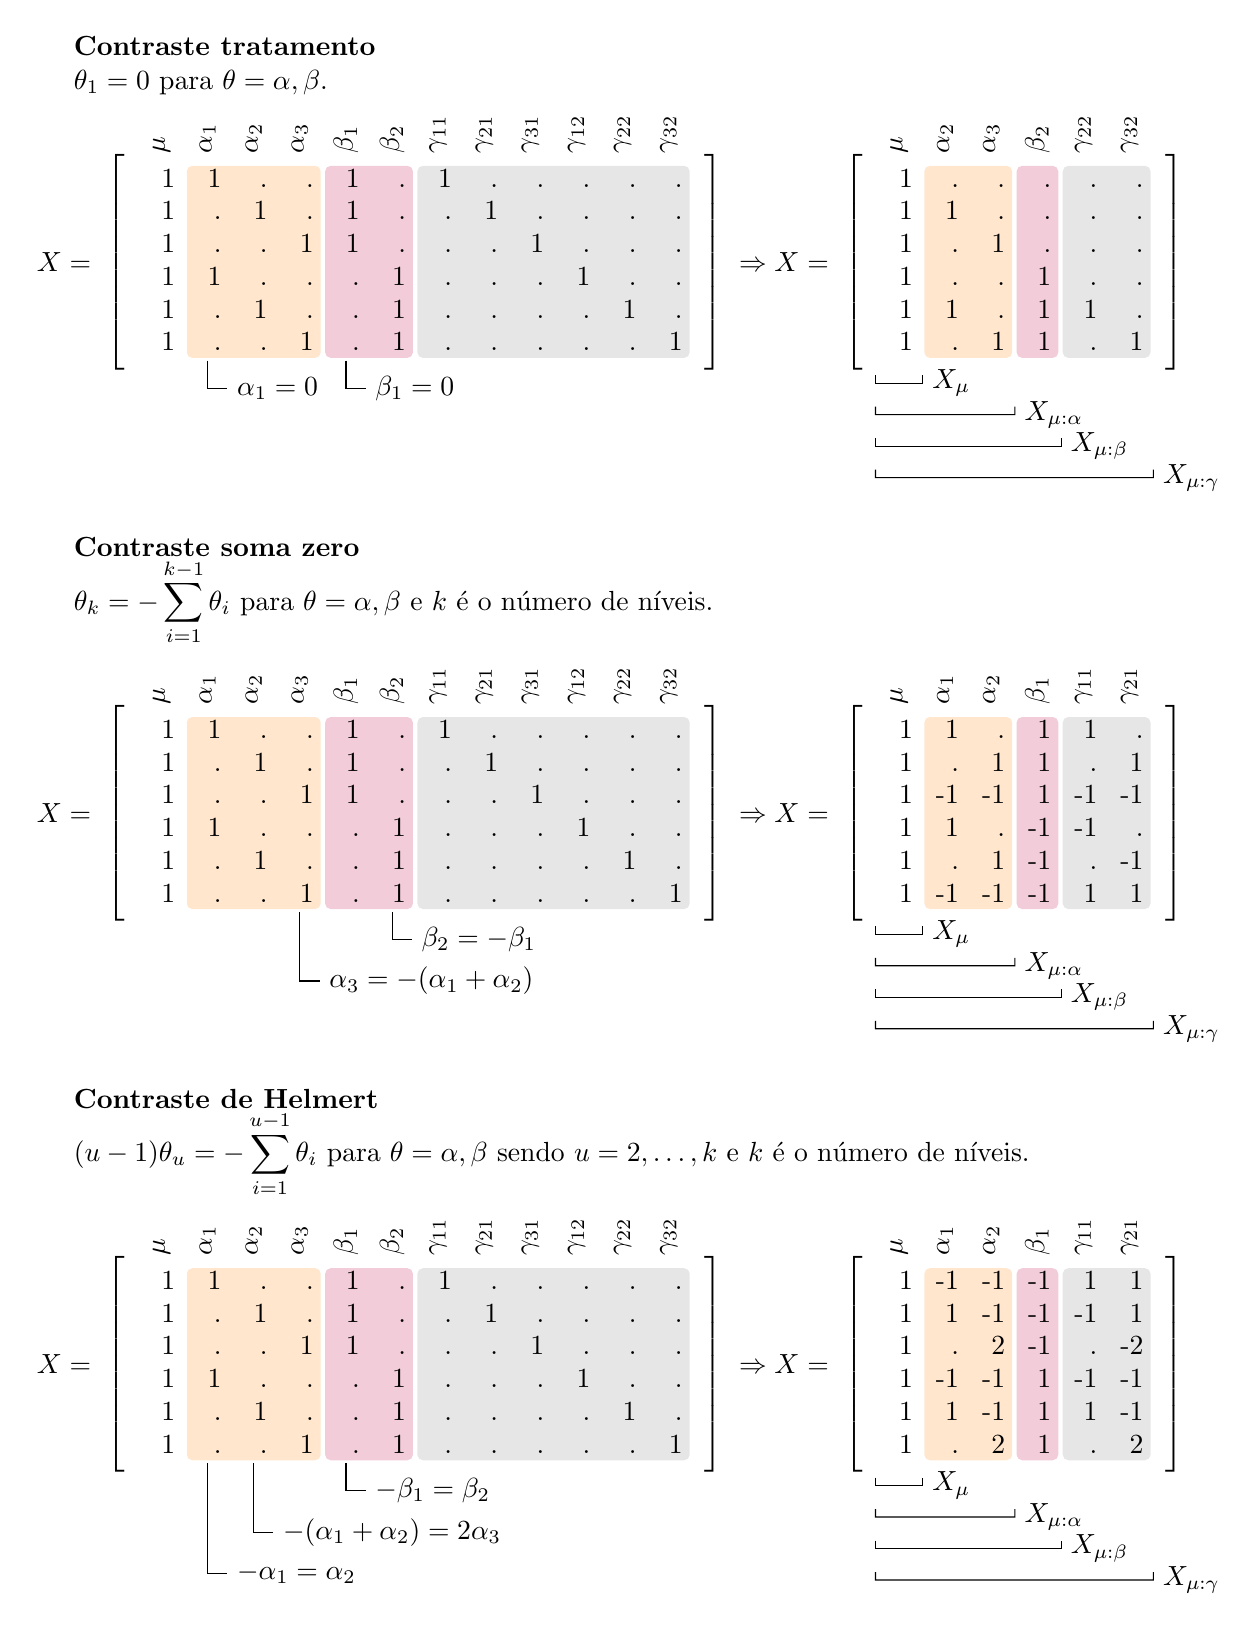
\begin{tikzpicture}[%
  mtx/.style = {
    matrix of math nodes,
    nodes in empty cells,
    left delimiter = {[},
    right delimiter = {]},
    every node/.style = {
      anchor = base,
      text width = 1em,
      text height = 1.2ex,
      align = right,
      anchor = base east
    }
  },
  hltr/.style = {opacity = 0.2, rounded corners = 2pt, inner sep = -1pt},
  txtup/.style = {rotate = 90, right},
  txtbt/.style = {yshift = -1ex}
]

\begin{scope}

  \matrix (X) at (0, 0) [mtx] {
    1 & 1 & . & . & 1 & . & 1 & . & . & . & . & . \\
    1 & . & 1 & . & 1 & . & . & 1 & . & . & . & . \\
    1 & . & . & 1 & 1 & . & . & . & 1 & . & . & . \\
    1 & 1 & . & . & . & 1 & . & . & . & 1 & . & . \\
    1 & . & 1 & . & . & 1 & . & . & . & . & 1 & . \\
    1 & . & . & 1 & . & 1 & . & . & . & . & . & 1 \\
  };

  \node[left=1em of X] (Xequal) {$X = $};
  \node[right=1em of X] (Xarrow) {$\Rightarrow X = $};

  \node[above=5em of Xequal, anchor = south west, align = left] {
    \textbf{Contraste tratamento}\\
    $\theta_1 = 0$ para $\theta = \alpha, \beta$.
  };

  % Efeitos.
  \node[txtup] at (X-1-1.north) {$\mu$};
  \node[txtup] at (X-1-2.north) {$\alpha_1$};
  \node[txtup] at (X-1-3.north) {$\alpha_2$};
  \node[txtup] at (X-1-4.north) {$\alpha_3$};
  \node[txtup] at (X-1-5.north) {$\beta_1$};
  \node[txtup] at (X-1-6.north) {$\beta_2$};
  \node[txtup] at (X-1-7.north) {$\gamma_{11}$};
  \node[txtup] at (X-1-8.north) {$\gamma_{21}$};
  \node[txtup] at (X-1-9.north) {$\gamma_{31}$};
  \node[txtup] at (X-1-10.north) {$\gamma_{12}$};
  \node[txtup] at (X-1-11.north) {$\gamma_{22}$};
  \node[txtup] at (X-1-12.north) {$\gamma_{32}$};

  % Restricoes.
  \draw (X-6-2.south) |- +(0.25, -1em) node[right] {$\alpha_1 = 0$};
  \draw (X-6-5.south) |- +(0.25, -1em) node[right] {$\beta_1 = 0$};

  % Colunas de efeitos.
  \begin{scope}[on background layer]
  \node[hltr, fill = orange, fit = (X-1-2)(X-6-4)] {};
  \node[hltr, fill = purple, fit = (X-1-5)(X-6-6)] {};
  \node[hltr, fill = gray,   fit = (X-1-7)(X-6-12)] {};
  \end{scope}

  \matrix (XX) [mtx, right = 1em of Xarrow] {
  1 & . & . & . & . & . \\
  1 & 1 & . & . & . & . \\
  1 & . & 1 & . & . & . \\
  1 & . & . & 1 & . & . \\
  1 & 1 & . & 1 & 1 & . \\
  1 & . & 1 & 1 & . & 1 \\
  };

  % Efeitos.
  \node[txtup] at (XX-1-1.north) {$\mu$};
  \node[txtup] at (XX-1-2.north) {$\alpha_2$};
  \node[txtup] at (XX-1-3.north) {$\alpha_3$};
  \node[txtup] at (XX-1-4.north) {$\beta_2$};
  \node[txtup] at (XX-1-5.north) {$\gamma_{22}$};
  \node[txtup] at (XX-1-6.north) {$\gamma_{32}$};

  % Colunas de efeitos.
  \begin{scope}[on background layer]
  \node[hltr, fill = orange, fit = (XX-1-2)(XX-6-3)] {};
  \node[hltr, fill = purple, fit = (XX-1-4)(XX-6-4)] {};
  \node[hltr, fill = gray,   fit = (XX-1-5)(XX-6-6)] {};
  \end{scope}

  \draw ($(XX-6-1.west)+(0, -.40)$) |- +(0, -0.1) -- ($(XX-6-1.east)+(0, -.50)$) node[right] {$X_{\mu}$} -- +(0, 0.1);

  \draw ($(XX-6-1.west)+(0, -.80)$) |- +(0, -0.1) -- ($(XX-6-3.east)+(0, -.90)$) node[right] {$X_{\mu:\alpha}$} -- +(0, 0.1);
  \draw ($(XX-6-1.west)+(0, -1.2)$) |- +(0, -0.1) -- ($(XX-6-4.east)+(0, -1.3)$) node[right] {$X_{\mu:\beta}$} -- +(0, 0.1);
  \draw ($(XX-6-1.west)+(0, -1.6)$) |- +(0, -0.1) -- ($(XX-6-6.east)+(0, -1.7)$) node[right] {$X_{\mu:\gamma}$} -- +(0, 0.1);

\end{scope}


\begin{scope}[yshift = -7cm]

  \matrix (X) at (0, 0) [mtx] {
    1 & 1 & . & . & 1 & . & 1 & . & . & . & . & . \\
    1 & . & 1 & . & 1 & . & . & 1 & . & . & . & . \\
    1 & . & . & 1 & 1 & . & . & . & 1 & . & . & . \\
    1 & 1 & . & . & . & 1 & . & . & . & 1 & . & . \\
    1 & . & 1 & . & . & 1 & . & . & . & . & 1 & . \\
    1 & . & . & 1 & . & 1 & . & . & . & . & . & 1 \\
  };

  \node[left=1em of X] (Xequal) {$X = $};
  \node[right=1em of X] (Xarrow) {$\Rightarrow X = $};

  \node[above=5em of Xequal, anchor = south west, align = left] {
    \textbf{Contraste soma zero}\\
    $\theta_k = -\displaystyle\sum_{i = 1}^{k - 1} \theta_i$ para $\theta = \alpha, \beta$
    e $k$ {\' e} o n{\' u}mero de n{\' i}veis.
  };

  % Efeitos.
  \node[txtup] at (X-1-1.north) {$\mu$};
  \node[txtup] at (X-1-2.north) {$\alpha_1$};
  \node[txtup] at (X-1-3.north) {$\alpha_2$};
  \node[txtup] at (X-1-4.north) {$\alpha_3$};
  \node[txtup] at (X-1-5.north) {$\beta_1$};
  \node[txtup] at (X-1-6.north) {$\beta_2$};
  \node[txtup] at (X-1-7.north) {$\gamma_{11}$};
  \node[txtup] at (X-1-8.north) {$\gamma_{21}$};
  \node[txtup] at (X-1-9.north) {$\gamma_{31}$};
  \node[txtup] at (X-1-10.north) {$\gamma_{12}$};
  \node[txtup] at (X-1-11.north) {$\gamma_{22}$};
  \node[txtup] at (X-1-12.north) {$\gamma_{32}$};

  % Restricoes.
  \draw (X-6-4.south) |- +(0.25, -2.5em) node[right] {$\alpha_3 = -(\alpha_1 + \alpha_2)$};
  \draw (X-6-6.south) |- +(0.25, -1em) node[right] {$\beta_2 = -\beta_1$};

  % Colunas de efeitos.
  \begin{scope}[on background layer]
  \node[hltr, fill = orange, fit = (X-1-2)(X-6-4)] {};
  \node[hltr, fill = purple, fit = (X-1-5)(X-6-6)] {};
  \node[hltr, fill = gray,   fit = (X-1-7)(X-6-12)] {};
  \end{scope}

  \matrix (XX) [mtx, right = 1em of Xarrow] {
  1 & 1 & . & 1 & 1 & . \\
  1 & . & 1 & 1 & . & 1 \\
  1 & -1 & -1 & 1 & -1 & -1 \\
  1 & 1 & . & -1 & -1 & . \\
  1 & . & 1 & -1 & . & -1 \\
  1 & -1 & -1 & -1 & 1 & 1 \\
  };

  % Efeitos.
  \node[txtup] at (XX-1-1.north) {$\mu$};
  \node[txtup] at (XX-1-2.north) {$\alpha_1$};
  \node[txtup] at (XX-1-3.north) {$\alpha_2$};
  \node[txtup] at (XX-1-4.north) {$\beta_1$};
  \node[txtup] at (XX-1-5.north) {$\gamma_{11}$};
  \node[txtup] at (XX-1-6.north) {$\gamma_{21}$};

  % Colunas de efeitos.
  \begin{scope}[on background layer]
  \node[hltr, fill = orange, fit = (XX-1-2)(XX-6-3)] {};
  \node[hltr, fill = purple, fit = (XX-1-4)(XX-6-4)] {};
  \node[hltr, fill = gray,   fit = (XX-1-5)(XX-6-6)] {};
  \end{scope}

  \draw ($(XX-6-1.west)+(0, -.40)$) |- +(0, -0.1) -- ($(XX-6-1.east)+(0, -.50)$) node[right] {$X_{\mu}$} -- +(0, 0.1);

  \draw ($(XX-6-1.west)+(0, -.80)$) |- +(0, -0.1) -- ($(XX-6-3.east)+(0, -.90)$) node[right] {$X_{\mu:\alpha}$} -- +(0, 0.1);
  \draw ($(XX-6-1.west)+(0, -1.2)$) |- +(0, -0.1) -- ($(XX-6-4.east)+(0, -1.3)$) node[right] {$X_{\mu:\beta}$} -- +(0, 0.1);
  \draw ($(XX-6-1.west)+(0, -1.6)$) |- +(0, -0.1) -- ($(XX-6-6.east)+(0, -1.7)$) node[right] {$X_{\mu:\gamma}$} -- +(0, 0.1);

\end{scope}


\begin{scope}[yshift = -14cm]

  \matrix (X) at (0, 0) [mtx] {
    1 & 1 & . & . & 1 & . & 1 & . & . & . & . & . \\
    1 & . & 1 & . & 1 & . & . & 1 & . & . & . & . \\
    1 & . & . & 1 & 1 & . & . & . & 1 & . & . & . \\
    1 & 1 & . & . & . & 1 & . & . & . & 1 & . & . \\
    1 & . & 1 & . & . & 1 & . & . & . & . & 1 & . \\
    1 & . & . & 1 & . & 1 & . & . & . & . & . & 1 \\
  };

  \node[left=1em of X] (Xequal) {$X = $};
  \node[right=1em of X] (Xarrow) {$\Rightarrow X = $};

  \node[above=5em of Xequal, anchor = south west, align = left] {
    \textbf{Contraste de Helmert}\\
    $(u - 1) \theta_u = -\displaystyle\sum_{i = 1}^{u - 1} \theta_i$ para $\theta = \alpha, \beta$
    sendo $u = 2, \ldots, k$ e $k$ {\' e} o n{\' u}mero de n{\' i}veis.
  };

  % Efeitos.
  \node[txtup] at (X-1-1.north) {$\mu$};
  \node[txtup] (alpha1) at (X-1-2.north) {$\alpha_1$};
  \node[txtup] (alpha2) at (X-1-3.north) {$\alpha_2$};
  \node[txtup] at (X-1-4.north) {$\alpha_3$};
  \node[txtup] (beta1) at (X-1-5.north) {$\beta_1$};
  \node[txtup] at (X-1-6.north) {$\beta_2$};
  \node[txtup] at (X-1-7.north) {$\gamma_{11}$};
  \node[txtup] at (X-1-8.north) {$\gamma_{21}$};
  \node[txtup] at (X-1-9.north) {$\gamma_{31}$};
  \node[txtup] at (X-1-10.north) {$\gamma_{12}$};
  \node[txtup] at (X-1-11.north) {$\gamma_{22}$};
  \node[txtup] at (X-1-12.north) {$\gamma_{32}$};

  % Restricoes.
  \draw (X-6-2.south) |- +(0.25, -4.0em) node[right] {$-\alpha_1 = \alpha_2$};
  \draw (X-6-3.south) |- +(0.25, -2.5em) node[right] {$-(\alpha_1 + \alpha_2) = 2\alpha_3$};
  \draw (X-6-5.south) |- +(0.25, -1.0em) node[right] {$-\beta_1 = \beta_2$};

  % Colunas de efeitos.
  \begin{scope}[on background layer]
  \node[hltr, fill = orange, fit = (X-1-2)(X-6-4)] {};
  \node[hltr, fill = purple, fit = (X-1-5)(X-6-6)] {};
  \node[hltr, fill = gray,   fit = (X-1-7)(X-6-12)] {};
  \end{scope}

  \matrix (XX) [mtx, right = 1em of Xarrow] {
    1 & -1 & -1 & -1 & 1 & 1 \\
    1 & 1 & -1 & -1 & -1 & 1 \\
    1 & . & 2 & -1 & . & -2 \\
    1 & -1 & -1 & 1 & -1 & -1 \\
    1 & 1 & -1 & 1 & 1 & -1 \\
    1 & . & 2 & 1 & . & 2 \\
  };

  % Efeitos.
  \node[txtup] at (XX-1-1.north) {$\mu$};
  \node[txtup] at (XX-1-2.north) {$\alpha_1$};
  \node[txtup] at (XX-1-3.north) {$\alpha_2$};
  \node[txtup] at (XX-1-4.north) {$\beta_1$};
  \node[txtup] at (XX-1-5.north) {$\gamma_{11}$};
  \node[txtup] at (XX-1-6.north) {$\gamma_{21}$};

  % Colunas de efeitos.
  \begin{scope}[on background layer]
  \node[hltr, fill = orange, fit = (XX-1-2)(XX-6-3)] {};
  \node[hltr, fill = purple, fit = (XX-1-4)(XX-6-4)] {};
  \node[hltr, fill = gray,   fit = (XX-1-5)(XX-6-6)] {};
  \end{scope}

  \draw ($(XX-6-1.west)+(0, -.40)$) |- +(0, -0.1) -- ($(XX-6-1.east)+(0, -.50)$) node[right] {$X_{\mu}$} -- +(0, 0.1);

  \draw ($(XX-6-1.west)+(0, -.80)$) |- +(0, -0.1) -- ($(XX-6-3.east)+(0, -.90)$) node[right] {$X_{\mu:\alpha}$} -- +(0, 0.1);
  \draw ($(XX-6-1.west)+(0, -1.2)$) |- +(0, -0.1) -- ($(XX-6-4.east)+(0, -1.3)$) node[right] {$X_{\mu:\beta}$} -- +(0, 0.1);
  \draw ($(XX-6-1.west)+(0, -1.6)$) |- +(0, -0.1) -- ($(XX-6-6.east)+(0, -1.7)$) node[right] {$X_{\mu:\gamma}$} -- +(0, 0.1);

\end{scope}

\end{tikzpicture}%
\end{document}